\documentclass{article}

\usepackage[dblblindworkshop]{neurips_2026}
\workshoptitle{AI Foundations for Power Grids: From Models to Deployment at Scale}

\usepackage[utf8]{inputenc}
\usepackage[T1]{fontenc}
\usepackage{hyperref}
\usepackage{url}
\usepackage{booktabs}
\usepackage{amsmath}
\usepackage{amsfonts}
\usepackage{graphicx}
\usepackage{microtype}
\usepackage{xcolor}

\title{Adaptive Expert Routing for Community Load Tracking:\\Stability Gains and Failure Modes}

% The workshop uses double-blind review. Do not add names, affiliations,
% acknowledgments, grant identifiers, or identifying repository links here.
\author{Anonymous Author(s)}

\begin{document}
\maketitle

\begin{abstract}
Grouped parameter sharing makes multi-agent reinforcement learning (MARL)
tractable for heterogeneous building portfolios, but permanently assigning a
building to one policy actor ignores that its flexibility changes with state.
We study this restriction on the 25-home IEA EBC Annex~96 Common Exercise~1
load-tracking task in CityLearn. We introduce a state-conditioned Soft Router
over five complete, communication-aware MAPPO actor experts. A staged procedure
first trains the router while freezing pretrained experts, then freezes the
router and adapts only action heads. Across three router seeds initialized from
one fixed-expert checkpoint, the resulting controller obtains
$45.12\pm0.35\%$ CV-RMSE, $3.78\pm0.44\,^{\circ}$C h per building-day, and
$17.30\pm1.33\%$ comfort exceedance. Relative to its fixed checkpoint, routing
improves mean comfort severity by 16.4\% while keeping CV-RMSE within 0.5
percentage points. The evaluation also exposes limits hidden by aggregate
metrics: the worst-building violation duration rises from 493 to
$569\pm17$ hours, joint router--expert adaptation concentrates 51.7\% of
traffic on one expert, and one branch becomes almost unused even under the
stable schedule. These results position adaptive routing as a useful but
incomplete enhancement to fixed grouping and illustrate why portfolio-level
accuracy alone is insufficient evidence for grid-interactive control.
\end{abstract}

\section{Introduction}

Aggregators can coordinate batteries and heating, ventilation, and air
conditioning (HVAC) across a community to track a portfolio-level reference
load. The learning problem is intrinsically multi-agent: each home has distinct
demand, thermal state, and flexibility, while success is measured at both the
portfolio and building levels. CityLearn provides a reproducible environment
for this setting \citep{citylearn2020,citylearnv2}, and recent work has shown
the promise of MARL for residential flexibility \citep{charbonnier2025,wilk2024}.
Yet a component that improves mean load tracking can still create unacceptable
local comfort violations, and a policy that is stable in one seasonal regime
may fail under another. This makes evaluation design as important as aggregate
reward.

Our starting point is grouped MAPPO \citep{mappo2022}: buildings are clustered
from physical and demand features, and members of a cluster share an actor.
Grouping reduces the number of independent policies and encourages transfer,
but creates a permanent building-to-actor assignment. Earlier experiments in
this project established that communication and grouping are not neutral
implementation details. Replacing the original TarMAC fusion
\citep{tarmac2019} with a compressed local projection and residual update
reduced Vermont CV-RMSE from 49.65\% to 47.01\% in a matched run, while changing
the clustering method or feature set materially altered both tracking and
comfort. A compact feature set---battery capacity, mean heating demand, and mean
non-shiftable load (3fA)---was the most stable fixed-group compromise.
Our router brings the conditional-computation idea of mixture-of-experts models
\citep{puigcerver2024softmoe,obandoceron2024moerl} to this grouped control
setting, where each expert is a complete closed-loop policy rather than a
feed-forward sublayer.

We ask whether actor selection should remain fixed after this useful prior has
been learned. Our contributions are:
\begin{itemize}
  \item a Soft Router that selects a \emph{complete} encoder--communication--head
  expert for every building and time step, avoiding incompatible latent spaces;
  \item a staged PPO training schedule with a fixed-group prior, entropy and
  load-balancing regularization, router-only learning, and low-rate head-only
  adaptation; and
  \item an evaluation that reports multi-seed mean performance, system-level
  effects, worst-building comfort, routing concentration, unsuccessful router
  variants, and a separately trained cross-climate stress test.
\end{itemize}
The main conclusion is deliberately qualified: stable routing improves the
mean tracking--comfort trade-off, but does not remove dependence on strong
pretrained groups and does not guarantee good tail comfort.

\section{Method}

\paragraph{Task and reward.}
At hour $t$, $N=25$ homes jointly track reference power $r_t$. Let
$y_t$ be aggregate net load, $e_t=y_t-r_t$, and let $d_{i,t}$ be home $i$'s
temperature distance outside the seasonal comfort interval. Training uses the
running normalized bias and tracking terms
\begin{equation}
B_t=\left|\frac{\sum_{\tau\leq t}e_\tau}{\sum_{\tau\leq t}r_\tau}\right|,
\qquad
E_t=\frac{\sqrt{t^{-1}\sum_{\tau\leq t}e_\tau^2}}
{t^{-1}\sum_{\tau\leq t}r_\tau},
\end{equation}
and a per-building reward
\begin{equation}
R_{i,t}=-\left[\frac{w_BB_t+w_EE_t}{N}+
w_C\left(w_I\mathbb{1}[d_{i,t}>0]+w_dd_{i,t}\right)\right].
\label{eq:reward}
\end{equation}
The shared terms promote portfolio tracking; the local term exposes comfort
costs that an aggregate objective can otherwise hide.

\paragraph{Fixed experts and communication.}
We standardize 3fA over the training homes and use Ward agglomerative clustering
\citep{ward1963} to construct five actor groups. Each expert follows the
centralized-training/decentralized-execution MAPPO backbone. Before actions are
formed, a one-round global TarMAC block communicates across all buildings. For
hidden state $h_i$, queries, keys, and values yield
$c_i=\sum_j\mathrm{softmax}_j(q_i^\top k_j/\sqrt{d_k})v_j$.
The hybrid fusion compresses the 256-dimensional local state to 64 dimensions,
combines it with the 64-dimensional message, and adds a residual update to the
original state. The fixed 3fA actors are trained for 500 episodes and provide
the router's expert checkpoint.

\paragraph{State-conditioned full-expert routing.}
For building $i$, the originally assigned encoder and global communication
module produce a 256-dimensional summary $h_{it}$. We append seven physical
quantities: normalized battery capacity and HVAC rating, state of charge (SOC),
available charging space, available discharge energy, non-shiftable load, and
heating demand. A shared $263\!\rightarrow\!64\!\rightarrow\!5$ network gives
\begin{equation}
d_{it}=\operatorname{softmax}(f_\theta([h_{it};q_{it}])/\tau),\qquad
g_{it}=(1-\alpha)p_i+\alpha d_{it},
\label{eq:gate}
\end{equation}
where $p_i$ is the one-hot fixed assignment. During training an expert is
sampled from $g_{it}$; deterministic evaluation uses its largest component.
Crucially, routing switches the matched encoder, communication branch, and
action head together. Switching only heads can feed them representations from
encoders on which they were never trained.

If expert $k$ defines action distribution $\pi_{\phi_k}$, the routed policy is
the mixture
\begin{equation}
\pi_{\theta,\phi}(a_{it}\mid s_t)=\sum_{k=1}^{5}g_{itk}(\theta)
\pi_{\phi_k}(a_{it}\mid s_t).
\label{eq:mixture}
\end{equation}
Thus PPO \citep{ppo2017} can update $\theta$ even when $\phi$ is frozen: the
likelihood of an executed action still depends on the gate. We add policy
entropy and
$\mathcal{L}_{\mathrm{bal}}=5^{-1}\sum_k(\bar g_k-\bar p_k)^2$, where $\bar p$
is the original group proportion.

\paragraph{Stable schedule.}
The router uses $\tau=0.5$, $\alpha:0.5\rightarrow1$ over 150 episodes, learning
rate $10^{-4}$, entropy scale 0.05, and balance coefficient 0.01. For episodes
1--500 all expert parameters are frozen. For episodes 501--1000 the router,
encoders, and communication module are frozen and only action heads adapt at
$10^{-5}$. This removes the moving target created when both router semantics and
expert behavior change simultaneously.

\section{Evaluation}

\paragraph{Protocol and metrics.}
Vermont uses January for training and February for testing, at one-hour
resolution; the comfort interval is $20$--$24^{\circ}$C. We report CV-RMSE,
absolute NMBE, comfort-exceedance rate, and comfort severity
$\mathrm{DH}_{bd}=\sum_{i,t}d_{i,t}\Delta t/(N D_{\mathrm{test}})$.
All are lower-is-better. Five independent seeds summarize the fixed 3fA family.
The final router uses three router-training seeds (0, 1, 42), but all start from
the same seed-42 fixed checkpoint. Table~\ref{tab:main} therefore includes both
the multi-seed family and the exact anchor; the routed and five-seed rows should
not be interpreted as fully independent end-to-end seed comparisons.

\begin{table}[t]
\centering
\small
\resizebox{\textwidth}{!}{%
\begin{tabular}{lrrrrrr}
\toprule
Controller & Runs & CV-RMSE (\%) & $|$NMBE$|$ (\%) & $\mathrm{DH}_{bd}$ & Comfort (\%) & Worst home (h) \\
\midrule
Fixed 3fA family & 5 & $49.86\pm3.65$ & $0.81\pm0.68$ & $4.64\pm1.27$ & $19.21\pm2.85$ & $471\pm68$ \\
Fixed seed-42 anchor & 1 & 44.62 & 0.57 & 4.52 & 20.07 & 493 \\
Stable full-expert router & 3 & $45.12\pm0.35$ & $1.35\pm0.33$ & $\mathbf{3.78\pm0.44}$ & $\mathbf{17.30\pm1.33}$ & $569\pm17$ \\
\bottomrule
\end{tabular}}
\caption{Vermont February test results. ``Worst home'' is the largest number
of comfort-violation hours among the 25 buildings. Router runs share the same
fixed seed-42 expert checkpoint.}
\label{tab:main}
\end{table}

\paragraph{Mean and system-level effects.}
Against its exact fixed anchor, the stable router reduces degree-hours by
16.4\% and comfort-exceedance rate by 13.8\%, while CV-RMSE increases only 0.50
percentage points. Across the broader fixed family, routing also has a lower
mean CV-RMSE, but this comparison benefits from starting all routers from the
strong seed-42 checkpoint. Absolute bias worsens from 0.57\% at the anchor to
$1.35\pm0.33\%$, exposing a real tracking--comfort trade-off. Downstream grid
metrics are mixed: the router's mean monthly peak falls from 281.9 to
276.2~kW and ramping from 487.2 to 476.5~kW, while site energy rises from
70.76 to 72.36~MWh. Load-share fairness is essentially unchanged (Gini 0.1438
versus $0.1435\pm0.0126$).

\paragraph{Ablations.}
The progression in Figure~\ref{fig:progression} shows that a good router cannot
be obtained merely by adding a gate. End-to-end training has acceptable
CV-RMSE (47.60\%) but poor comfort severity (10.02 $^{\circ}$C h/building-day).
A shared-encoder three-stage model is worse still (52.44\% CV-RMSE and 31.35\%
comfort exceedance). Preserving complete expert branches improves CV-RMSE to
45.45\%; freezing the learned router and restricting subsequent adaptation to
the heads gives the final stable result. Full numerical ablations are in
Appendix~\ref{app:ablations}.

\begin{figure}[t]
  \centering
  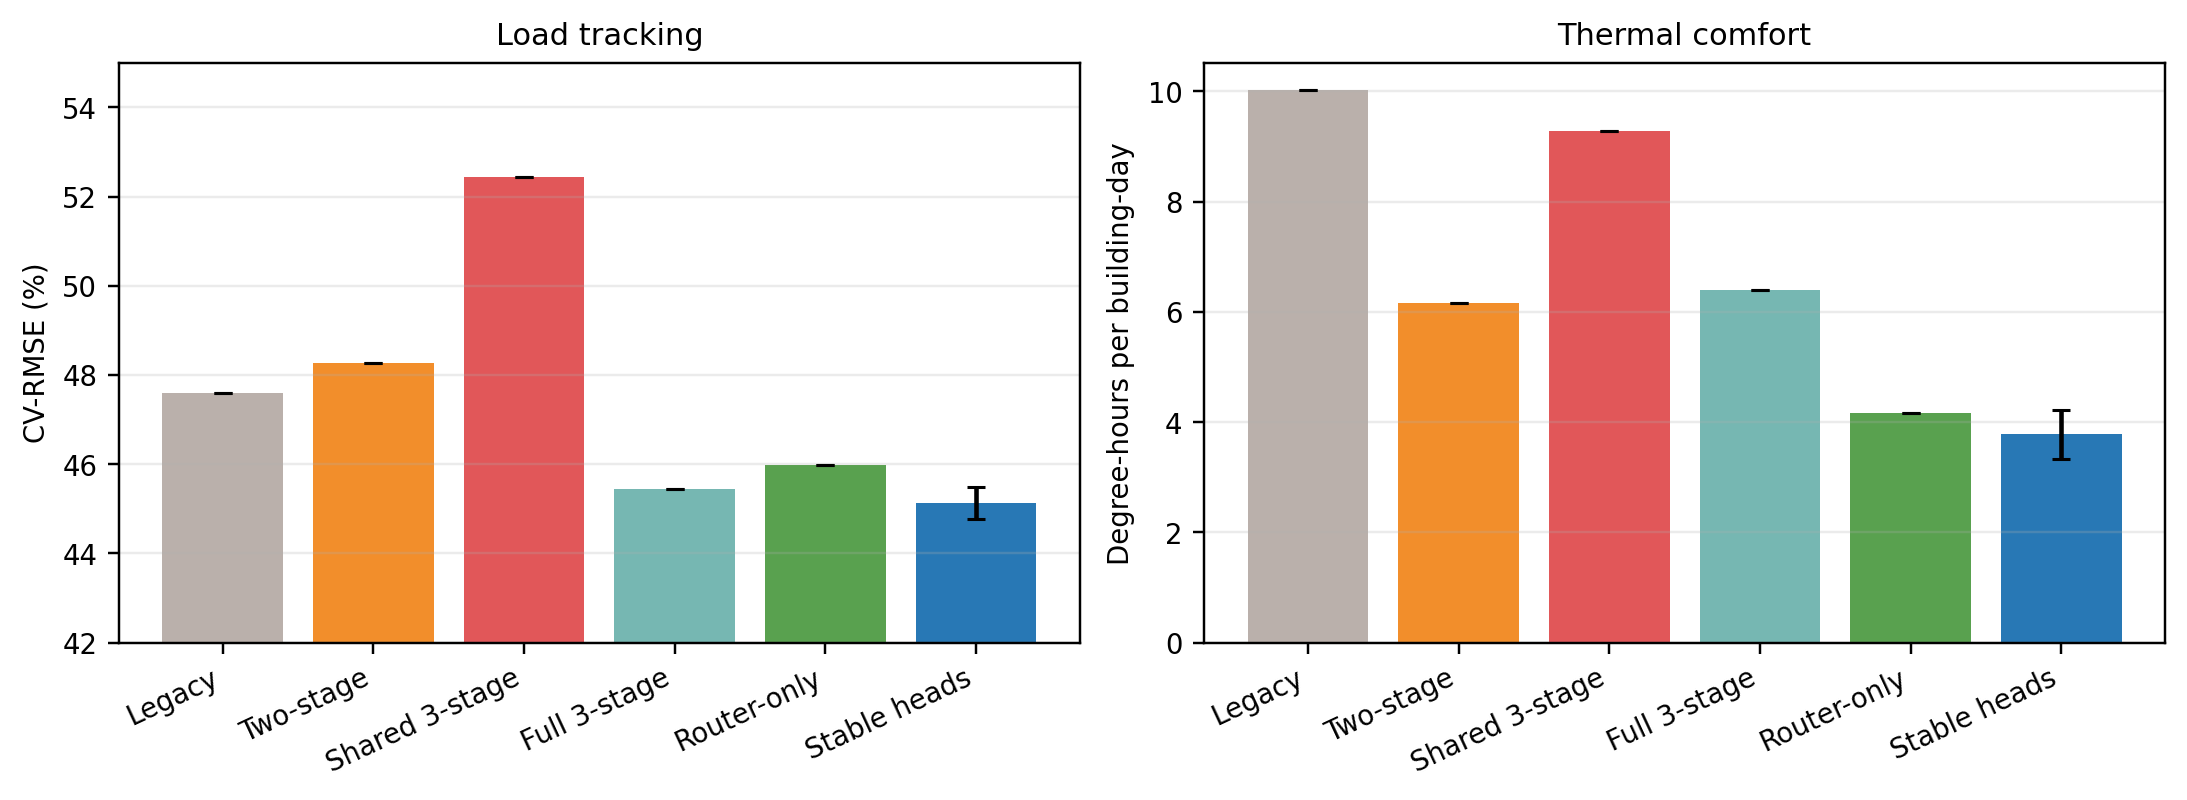
\includegraphics[width=0.88\linewidth]{figures/soft_router_progression.png}
  \caption{Soft-router development stages. Lower is better on every panel;
  the final bar reports the three-seed stable-head mean.}
  \label{fig:progression}
\end{figure}

\section{Failure modes, regime shift, and limitations}

\paragraph{Routing collapse.}
After 500 router-only episodes, the largest expert share is 36.4\%. Continuing
joint full-expert adaptation reduces gate entropy from 0.275 to 0.171 and sends
51.7\% of decisions to one expert. Freezing the router during head adaptation
preserves entropy at 0.276 and limits the largest share to 37.0\%. Nevertheless,
one expert receives only 0.015--0.036\% of final traffic across the three stable
runs. Entropy and balance penalties prevent complete one-expert collapse, not
expert under-use.

\paragraph{Aggregate gains hide local risk.}
The stable router improves average comfort but raises the worst-building
violation duration from 493 hours at its anchor to $569\pm17$ hours. The
five-seed fixed family averages $471\pm68$ hours. This reversal is invisible in
CV-RMSE and portfolio mean comfort and is the strongest reason not to interpret
the method as deployment-ready. Explicit per-building constraints or a
tail-aware objective are needed before narrow autonomy.

\paragraph{Climate stress test.}
We separately retrain the 3fA design in Texas, replacing mean heating with mean
cooling demand and using August/September train/test months. It reduces CV-RMSE
to $78.83\pm4.90\%$, versus 163.74\% for no control and 207.63\% for the
rule-based controller, but retains a large $45.57\pm1.98\%$ absolute bias.
This tests transfer of the \emph{feature design}, not zero-shot transfer of a
Vermont policy; it therefore does not establish out-of-distribution policy
robustness.

\paragraph{Scope.}
All final router seeds reuse one unusually strong expert checkpoint, the study
contains only 25-building Vermont and Texas simulations, and CityLearn enforces
asset dynamics but contains no distribution-network or AC power-flow model.
Consequently we make no claim about voltage, line-flow, or contingency
feasibility. Future work should train complete expert--router systems from
independent initializations, evaluate unseen building portfolios and target
profiles, optimize tail comfort, and couple control to AC network constraints.

\section{Conclusion}

State-conditioned routing can relax a permanent building-to-actor assignment
without discarding useful grouped policies. The effective recipe is
conservative: route complete experts, learn selection against frozen reference
policies, and adapt only small output heads after the gate stabilizes. Its
benefits are meaningful at the portfolio mean, but the worst-building result
and residual expert under-use show why component accuracy is insufficient.
For grid-interactive MARL, router concentration and per-asset tails should be
reported alongside aggregate tracking metrics.

\section*{Generative AI disclosure}
A generative-AI system was used to assist with manuscript organization and
language editing. The authors verified the technical descriptions, numerical
results, and references against the implementation, recorded experiment
artifacts, and cited sources. Generative AI was not part of the research method
and did not generate experimental data or figures.

\bibliographystyle{plainnat}
\bibliography{references}

\appendix
\section{Router ablations and additional protocol}
\label{app:ablations}

\begin{table}[h]
\centering
\small
\resizebox{\textwidth}{!}{%
\begin{tabular}{llrrrr}
\toprule
Variant & Main change & CV-RMSE & $|$NMBE$|$ & $\mathrm{DH}_{bd}$ & Comfort \\
 & & (\%) & (\%) & ($^{\circ}$C h) & (\%) \\
\midrule
Legacy end-to-end & random policies, joint training & 47.60 & 4.31 & 10.02 & 24.64 \\
Two-stage freeze200 & pretrained experts & 48.26 & 1.35 & 6.15 & 21.76 \\
Two-stage prior0.7 & softer prior & 46.54 & 1.02 & 6.60 & 22.05 \\
Two-stage no capacity & remove seven router inputs & 46.94 & 0.57 & 5.53 & 19.54 \\
Three-stage shared & shared encoder & 52.44 & 7.48 & 9.27 & 31.35 \\
Three-stage full expert & preserve complete branches & 45.45 & 2.28 & 6.39 & 20.42 \\
Stable router-only & experts always frozen & 45.99 & 1.22 & 4.16 & 19.17 \\
Stable heads (3 seeds) & router freeze + head adaptation & $45.12\pm0.35$ & $1.35\pm0.33$ & $3.78\pm0.44$ & $17.30\pm1.33$ \\
\bottomrule
\end{tabular}}
\caption{Development ablation. Single-run rows use seed 42; only the final row
reports multiple router-training seeds.}
\end{table}

The MAPPO configuration uses actor and critic learning rates $3\times10^{-4}$,
$\gamma=0.99$, GAE $\lambda=0.95$, PPO clip 0.2, 10 PPO epochs, four mini-batches,
and 256-dimensional two-layer actors. The communication block uses 32-dimensional
queries/keys, 64-dimensional values, one global round, and a residual update.
The fixed actors and final router schedules each see complete one-month training
episodes. Evaluation is deterministic over the held-out following month. The
Vermont comfort interval is 20--24$^{\circ}$C; Texas uses 22--26$^{\circ}$C.

\section{Cross-climate feature-design stress test}

\begin{table}[h]
\centering
\small
\begin{tabular}{lrrrr}
\toprule
Climate/controller & CV-RMSE & $|$NMBE$|$ & $\mathrm{DH}_{bd}$ & Comfort \\
 & (\%) & (\%) & ($^{\circ}$C h) & (\%) \\
\midrule
Vermont 3fA & $49.64\pm1.59$ & $3.04\pm1.49$ & $5.10\pm1.95$ & $18.74\pm1.90$ \\
Texas 3fA & $78.83\pm4.90$ & $45.57\pm1.98$ & $1.59\pm0.31$ & $11.22\pm1.66$ \\
Texas no control & 163.74 & 79.12 & -- & -- \\
Texas rule based & 207.63 & 89.57 & -- & -- \\
\bottomrule
\end{tabular}
\caption{Three-seed 3fA role-based comparison. Vermont uses capacity--heating
mean--non-shiftable-load mean; Texas uses capacity--cooling mean--non-shiftable-load
mean and is retrained from scratch. Climate scales differ, so Vermont and Texas
rows should not be directly ranked.}
\end{table}

\clearpage
\section*{AI4PowerGrids domain checklist}
% 中文：
%   AI4PowerGrids 电网领域检查表

\begin{enumerate}
  \item \textbf{Physics feasibility.}
  \emph{Not applicable to AC power-flow feasibility.} CityLearn enforces the
  simulated battery, HVAC, and building thermal dynamics and bounds the control
  actions, while Section~4 and Appendices~B--C report thermal-comfort violations
  explicitly. The benchmark does not include a distribution-network model;
  consequently, voltage, line-flow, and full AC power-flow feasibility are not
  evaluated and no such claim is made.
  % 中文（物理可行性）：
  %   不适用于交流潮流可行性。CityLearn 会执行模拟电池、HVAC 和建筑热动态，
  %   并限制控制动作；第 4 节及附录 B--C 明确报告了室内热舒适度违规情况。
  %   该基准不包含配电网络模型，因此本文没有评估电压、线路潮流或完整交流潮流
  %   可行性，也不作出相关声明。

  \item \textbf{Out-of-distribution evaluation.}
  Section~5 and Appendix~D evaluate the same feature-design principle in two
  seasonal/climate regimes (Vermont heating and Texas cooling), each with a
  chronological held-out month. The Texas controller is retrained, so this is
  not zero-shot evaluation of one policy on an unseen climate or topology. This
  missing test is stated as a limitation.
  % 中文（分布外评估）：
  %   第 5 节和附录 D 在 Vermont 供暖季与 Texas 制冷季两种气候工况中评估
  %   同一套特征设计原则，并分别使用按时间顺序留出的测试月份。
  %   Texas 控制器经过重新训练，因此这不是将同一策略零样本部署到未见气候
  %   或拓扑上的评估；本文已将缺少这种测试明确列为局限。

  \item \textbf{Failure modes.}
  Section~4 reports the reversal between mean and worst-building comfort and
  the unequal numbers of training episodes. Appendices~B--C expose daily metric variation
  and persistent temperature violations in individual homes. Section~3 also
  explains why joint router/expert training was rejected after routing
  concentration and policy instability were observed.
  % 中文（失效模式）：
  %   第 4 节报告了平均舒适度与最差建筑舒适度之间的结论反转，以及各方法训练
  %   episode 数不同的问题。附录 B--C 展示逐日指标波动和个别住宅持续温度超限。
  %   第 3 节还说明：由于观察到路由集中和策略不稳定，最终没有采用路由器与
  %   专家联合训练方案。

  \item \textbf{System-level effect.}
  Section~4 and Appendix~A report portfolio CV-RMSE, NMBE, peak demand, and
  ramping together with building-level comfort. This evaluates each controller
  inside the complete closed-loop CityLearn portfolio rather than as a
  standalone predictor or router.
  % 中文（系统级影响）：
  %   第 4 节和附录 A 同时报告组合层面的 CV-RMSE、NMBE、峰值需求、ramping，
  %   以及建筑层面的舒适度。由此评估的是完整 CityLearn 建筑组合闭环中的控制器，
  %   而不是脱离系统的独立预测器或路由器。

  \item \textbf{Data and code.}
  The experiments use the open CityLearn implementation and IEA EBC Annex~96
  Common Exercise~1 benchmark data. We plan to provide the training and
  evaluation code, environment specifications, configuration scripts, processed
  metric tables, and plotting code as anonymized supplementary material during
  review, followed by a de-anonymized public repository upon acceptance.
  % 中文（数据与代码）：
  %   实验使用开放的 CityLearn 实现和 IEA EBC Annex 96 Common Exercise 1
  %   基准数据。我们计划在评审期间以匿名补充材料形式提供训练与评估代码、环境
  %   规格、配置脚本、处理后的指标表和绘图代码；若论文录用，再公开去匿名化后的
  %   代码仓库。
\end{enumerate}


\end{document}
